
\subsection{Sensordaten-Fusion}
\label{headtracking_fusion_subsec}
Die Sensordaten-Fusion beschreibt die Verknüpfung von mehreren Sensoren um Informationen besserer Qualität zu gewinnen. In diesem Projekt gilt des die aufbereiteten Daten aus beiden Gyroskopen, Beschleunigungsensor und Magenetometer derart zu fusioneieren, dass letztlich die zu ermittelnde \emph{Orientierung} des Kopfes möglichst exakt bestimmt werden kann. In den folgenden Abschnitten werden unterschiedliche Fusionsansätze dargestellt und entsprechend der Aufgabenstellung des Projekts bewertet. 

\subsubsection{Madgwick-Filter}
Die Filterung nach Madgwick \cite{madgwick2010efficient} gilt als neuartiger Ansatz zur Bestimmung der Orientierung basierend auf Gyroskop, Beschleunigungssensor und Magnetometer.
\todo{weiter ausführen}

Auch wenn der Madgwick-Filter bereits als fertige ROS-Node\todo{cite} vorhanden ist und  bessere Ergebnisse als der Kalman-Filter liefern soll, haben wir uns gegen den Madgwick-Filter entschieden, da das Optimierungsverfahren auf eine Darstellung über Quaternione basiert und dadurch der erzielte Mehrwert und erreichten Verbesserungen so nur schwer nachvollziehbar bzw. debuggbar gewesen sind. Außerdem war der Madgwick-Filter nur schwer an unsere bisherige Implementierung anpassbar.
\todo{Kann man so nicht stehen lassen, Begründung mit Quaternionen ist falsch. nutzen wir ja gerade beim Komplementär-Filter}

\subsubsection{Kalman-Filter}
Im ersten Schritt \emph{(Prädiktionsschritt)} des Kalman-Filters wird die zeitlich vorangegangene Schätzung als Grundlage genommen, um die Vorhersage für den aktuellen Zeitpunkt zu ermitteln. Der zweite Schritt \emph{(Korrektur- oder Innovationsschritt)} besteht daraus, die Vorhersagen mit neuen Informationen des aktuelle Messwerts zu korrigieren um somit die gesuchten Schätzwerte zu erreichen.

Um bei einer fehlerbehafteten Beobachtung den Systemzustand zu korrigieren müssen fehlerhafte Beobachtungen über mathematische Gleichungen beschreibbar und Fehlerverteilungen für Sensoren bekannt sein. Diese Informationen sind uns während der Bearbeitung des Projekts nicht bekannt gewesen. Infolgedessen haben wir beschlossen den hierfür benötigten Mehraufwand an Zeit und Ressourcen lieber in den bereits fortgeschrittenen Komplementär-Filter zu investieren.
\todo{weiterer Grund: Reagiert wohl langsamer auf Änderungen (Diskussion nach Abschlusspräsentation}

\subsubsection{Komplementär-Filter}
Nach Brooks und Iyengar \cite{} \todo{Cite} hat eine komplementäre Fusion das Ziel, die Genauigkeit von Daten zu verbessern. 
Dabei wirken die Sensoren unabhängig voneinander und liefern unterschiedliche Erkenntnisse und Sichtbereiche die Orientierung zu unterschiedlichen Zeiten verbessert.\todo{Satzbau}

Die Gyroskope sind wie bereits erwähnt bei einer langen Laufzeiten fehleranfällig und erzeugen einen Drift. 
Daher wird im ersten Schritt eine SLERP-Interpolation (Sperical Linear Interpolation) eingesetzt, die bei jedem Zeitschritt die Orientierung der Gyroskope zu $95\%$ und Orientierung des Beschleunigungssensor zu $5\%$ berücksichtigt. Hierbei wird das \emph{roll} und \emph{pitch} gestützt. Der zweite Schritt zielt auf die Verbesserung von \emph{yaw} ab. Eine weitere Interpolation verrechnet dieses Ergebnis mit den aufbereiteten Magnetometerwerten zu $5\%$ pro Zeitschritt. Formal lässt sich die Gewichtung folgendermaßen beschreiben:
\begin{equation}
    gyro.slerp(0.05, acc).slerp(0.05, mag)
\end{equation}
\todo{Formel in mathematische Formel umbauen, nicht Quellcode}


Eine Übersicht der Fusionierung mit dem Komplementär-Filter ist Abbildung \ref{fig:fusion_complementary} zu entnehmen.

\begin{figure}[ht]
	\begin{center}
		\scalebox{0.83}{
	\begin{tikzpicture}[%
		>=stealth, % Aussehen der Pfeilspitzen
		->, % Linien als Verbindungslinien
		looseness=.7, % Kr"ummung der Pfeile mit Option ’bent’
		auto, % Position des Ankers f"ur Node Labels
		color=black, % Farbe aller Linien
		%text=red, % Textfarbe in den Matrix-Nodes
		line width=1pt, % Linienst"arke f"ur alle Elemente
		text centered
	]
		\tikzstyle{every node}=[shape=rectangle,draw,fill=white,
		anchor=center] % Stil der Node-Beschriftung der
	\node[rectangle, rotate=-30, draw=orange, text width=2.5cm, outer sep=3pt, minimum size=1.5cm] at (0.6,4.5) {\textbf{$\alpha X+(1-\alpha)Y$}};
	\node[rectangle, font=\bfseries, double=green, text width=2.0cm, outer sep=3pt, minimum size=1.5cm](gyro) at (-7.0,5.5) {Gyro};
	\node[rectangle, font=\bfseries, double=green, text width=2.0cm, outer sep=3pt, minimum size=1.5cm](acc) at (-3.0,5.5) {Acc};
	
	\node[rectangle, font=\small, text width=2.5cm, outer sep=3pt, minimum size=1.5cm](interpol1) at (-3.0,2.5) {Interpolation \\ \textit{(SLERP)}};
	
	\node[rectangle, font=\small, text width=2.5cm, outer sep=3pt, minimum size=1.5cm](interpol2) at (-3.0,-2.5) {Interpolation \\ \textit{(SLERP)}};
	\node[rectangle, font=\bfseries, double=green, text width=2.0cm, outer sep=3pt, minimum size=1.5cm](mag) at (-7.0,-2.5) {Mag};
	
	\node[draw=none] at (-0.5, 0.5)(imageAbove) {\scalebox{0.33}{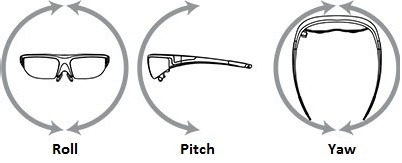
\includegraphics{rpy}}};
	\node[draw=none] at (-1.7, -0.5) {\scalebox{0.02}{
\includegraphics{Yes}}};
	\node[draw=none] at (-0.5, -0.5) {\scalebox{0.02}{
\includegraphics{Yes}}};
	\node[draw=none] at (0.75, -0.5) {\scalebox{0.02}{
\includegraphics{cross}}};
	
	\node[draw=none] at (1.0, -2.5)(imageBelow) {\scalebox{0.33}{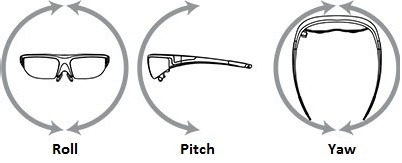
\includegraphics{rpy}}};
	\node[draw=none] at (-0.2, -3.5) {\scalebox{0.02}{
\includegraphics{Yes}}};
	\node[draw=none] at (1., -3.5) {\scalebox{0.02}{
\includegraphics{Yes}}};
	\node[draw=none] at (2.2, -3.5) {\scalebox{0.02}{
\includegraphics{Yes}}};

	\draw[orange, line width=2] (gyro) to[out=-90,in=-180] node[black, above, draw=none, fill=white, font=\small]{$0.95$} (interpol1);
	\draw[orange, line width=2] (acc) -- node[black, above, draw=none, fill=white, font=\small]{$0.05$} (interpol1);
	\draw[orange, line width=2] (interpol1) -- node[black, above, draw=none, fill=white, font=\small]{$0.95$} (interpol2);
	\draw[orange, line width=2] (mag) -- node[black, above, draw=none, fill=white, font=\small]{$0.05$} (interpol2);
	\draw[orange, line width=2] (interpol2) -- (imageBelow);
	
	\end{tikzpicture}}
	\end{center}
   \caption[]{Fusion -- Komplementärfilter}
   \label{fig:fusion_complementary}
\end{figure}